%编译环境:Windows 7+CTeX_2.9.2.164_Full+XeLaTeX
%文档编码:UTF-8
\documentclass[12pt,a4paper,landscape,fancyhdr,fntef,oneside]{ctexbook}
\usepackage{verbatim}
\usepackage{fancyvrb}
\usepackage{geometry}
\usepackage{tikz}
\usepackage[CJKbookmarks, colorlinks, bookmarksnumbered=true,pdfstartview=FitH,linkcolor=black,citecolor=black]{hyperref}
\usepackage{shortvrb}
\MakeShortVerb{\|}
\usepackage{graphicx}
% 设置图形文件的搜索路径
\graphicspath{{chapter/}{figure/}}
\newcommand\cs{
\begin{center}
  \S
\end{center}
}

\DefineVerbatimEnvironment{code}{Verbatim}%
  {frame=lines,framerule=0.5mm,rulecolor=\color{black},%
  fontseries=tt,xleftmargin=4mm,tabsize=4,numbers=left,numbersep=1.5mm}
\renewenvironment{quote}
                {\kaishu
                 \list{}{\rightmargin   2em
                         \listparindent 2em
                         \itemindent    2em
                         \parsep        0em}
                 \item\relax}
                {\endlist}

\CTEXsetup[name={第,天}]{chapter}
\CTEXsetup[number={\arabic{chapter}}]{chapter}
\setcounter{chapter}{-1}
\renewcommand\thesection{\arabic{section}}
\CTEXsetup[format+={\flushleft}]{section}

%%%%% Definitions
%%% Define a new command that prints the title only
\makeatletter							% Begin definition
\def\printtitle{%						% Define command: \printauthor
    {\huge {\@title}\par}}		% Typesetting
\makeatother							% End definition

\title{\hfill{\small \textbf{30日でできる! OS自作入門}}\\
\hfill \textbf{30天自制操作系统}\\
\hfill {\large\kaishu 读书笔记}}

%%% Define a new command that prints the author(s) only
\makeatletter							% Begin definition
\def\printauthor{%					% Define command: \printtitle
    {\large \@author}}				% Typesetting
\makeatother							% End definition

\author{
		\hfill 【日】川合秀実\quad 著\\	
		\hfill 周自恒~李黎明~曾祥江~张文旭\quad 译\\	
}

\renewcommand\maketitle{%
  \newpage
  \thispagestyle{empty}
  %%% Top of the page: Author, Title and Abstact

\begin{minipage}{0.48\linewidth}
	
	\vspace{.2\textheight}
	
\includegraphics[height=0.6\textheight]{Nekomata.jpg}\\	

\end{minipage} %\hspace{0pt}
%
\begin{minipage}{0.02\linewidth}
	\vspace{.2\textheight}
	\rule{3pt}{0.6\textheight}
\end{minipage} %\hspace{0pt}
%
\begin{minipage}{0.5\linewidth}
\begin{flushleft}
\vspace{.2\textheight}
\printtitle
\vspace{.2\textheight}
\printauthor
\end{flushleft}
\end{minipage}
%\vspace{20pt}		% Add some vertical spacing to seperate the abstract from the rest of the article
\clearpage}
\renewcommand\contentsname{目\hspace{2em}录}

\begin{document}
\maketitle

\newpage
\thispagestyle{empty}
{\hfil \huge \textbf{前\hspace{2em}言}}\par
\vspace{.1\textheight}
本文档为《30天自制操作系统》(人民邮电出版社)一书的读书笔记。\par

文档发布在Github上,将随着阅读进度不定期更新。请访问 https://github.com/mengyingchina/osask-notes 获取文档最新的版本。\par
\vspace{1em}
原书的版权声明一节,有:
\begin{quote}
本书中文简体字版由Mynavi Corporation授权人民邮电出版社独家出版。未经出版者书面许可,不得以任何方式复制或抄袭本书内容。
\end{quote}

由于部分内容摘自书中,不清楚这样摘录部分内容会不会存在版权问题,如果有版权问题,我会及时删除相关内容,请知情者告知\footnote{Email:mail@wanhu.me},谢谢!

\frontmatter
\tableofcontents

\mainmatter

\chapter{着手开发之前}

\section{	前言	}
\begin{quote}
阅读本书几乎不需要相关储备知识,这一点稍后还会详述。不管是用什么编程语言,只要是曾经写过简单的程序,对编程有一些感觉,就已经足够了(即使没有任何编程经验,应该也能看懂),因为这本书主要就是面向初学者的。书中虽然有很多C语言程序,但实际上并没有用到很高深的C语言知识,所以就算是曾经因为C语言太难而中途放弃的人也不用担心看不懂。当然,如果具备相关知识的话,理解起来会相对容易一些,不过即使没有相关知识也没关系,书中的说明都很仔细,大家可以放心。

本书以IBM PC/AT兼容机(也就是所谓的Windows个人电脑)为对象进行说明。
\end{quote}

\section{	何谓操作系统	}
\section{	开发操作系统的各种方法	}
\section{	无知则无畏	}

\begin{quote}
当我们打算开发操作系统时,总会有人从旁边跳出来,罗列出一大堆专业术语,问这问那,像内核怎么做啦,外壳怎么做啦,是不是单片啦,是不是微内核啦,等等。虽然有时候提这些问题也是有益的,但一上来就问这些,当然会让人无从回答。

要想给他们一个满意答复,让他们不再从旁指手画脚的话,还真得多学习,拿出点像模像样的见解才行。但我们是初学者,没有必要去学那些麻烦的东西,费时费力且不说,当我们知道现有操作系统在各方面都考虑得如此周密的时候,就会发现自己的想法太过简单而备受打击没了干劲。如果被前人的成果吓倒,只用这些现有的技术来做些拼拼凑凑的工作,岂不是太没意思了。

所以我们这次不去学习那些复杂的东西,直接着手开发。就算知道一大堆专业术语、专业理论,又有什么意思呢?还不如动手去做,就算做出来的东西再简单,起码也是自己的成果。而且自己先实际操作一次,通过实践找到其中的问题,再来看看是不是已经有了这些问题的解决方案,这样下来更能深刻地理解那些复杂理论。不管怎么说,反正目前我们也无法回答那些五花八门的问题,倒不如直接告诉在一旁指手画脚的人们:我们就是想用自己的方法做自己喜欢的事情,如果要讨论高深的问题,就另请高明吧。
\end{quote}

作者苦口婆心地说了这么多就是希望如果你想开发个操作系统,就动手去写吧,到底自己重写个操作系统有什么用倒可以先放着。

如果你到现在还对要不要读这本书,或者读这本书的期望的收获有疑问,推荐你阅读豆瓣上本书的一篇评论\footnote{ http://book.douban.com/review/5606888/ }后再自行决定。
\begin{quote}
这本书对基础知识要求不高,懂点C语言和CPU基本知识就可以了,适合初学者。要是奔着了解操作系统原理或内核的期望,就不适宜读这本书了。30天后也许你真的可以向作者那样做出一个基本的系统模型,但这并不意味着你对内存管理、进程管理、设备管理有着怎样高深的认识。读这本书之前先弄清自己的定位吧,毕竟时间宝贵。
\end{quote}

\section{	如何开发操作系统	}
\section{	操作系统开发中的困难	}
\section{	学习本书时的注意事项(重要!)	}
\section{	各章内容摘要	}


\chapter{	从计算机结构到汇编程序入门	}
\section{	先动手操作	}
\label{start}
随书附带了光盘\footnote{下载链接:http://pan.baidu.com/share/link?shareid=541099\&uk=3657658273 或自行搜索“30天自制操作系统.iso”},给出了书中的全部示例程序,以及部分用到的工具。
\begin{quote}
打开附带光盘,里面有一个名为tolset的文件夹,把这个文件夹复制到硬盘的任意一个位置上。现在里面的东西还不多,只有3MB左右,不过以后我们自己开发的软件也都要放到这个文件夹里,所以往后它会越来越大,因此硬盘上最好留出100MB左右的剩余空间。工具安装到此结束,我们既不用修改注册表,也不用设定路径参数,就这么简单。而且以后不管什么时候,都可以把这整个文件夹移动到任何其他地方。用这些工具,我们不仅可以开发操作系统,还可以开发简单的Windows应用程序或OSASK应用程序等。
\end{quote}

示例程序在附带光盘中名为projects的目录下,只要需要的示例程序目录复制到tolset文件夹里,就可以正常运行示例程序了。

考虑到开发中使用真实的软盘很不方便,作者特意准备了一个模拟器。

\begin{quote}
我们有了这个模拟器,不用软盘,也不用终止Windows,就可以确认所开发的操作系统启动以后的动作,很方便呢。

使用模拟器的方法也非常简单,我们只需要在用!cons\_nt.bat\footnote{要根据Windows的版本决定用哪一个。后缀为9x代表是Windows 9X系统,后缀为nt的代表使用NT 架构的Windows 系统,如Windows XP 及其以后的版本,以后默认为运行cons\_nt.bat,并在后面将其简写为!cons。\par
PS:作者开发这个系统是2000年左右的事情,写书的时间也比较早,所以考虑了这些问题,可以理解哈!}(或者是!cons\_9x.bat)打开的命令行窗口中输入“run” 指令就可以了。然后一个名叫QEMU 的非常优秀的免费PC 模拟器就会自动运行。
\end{quote}

\cs

在这一节中,作者使用二进制编辑器(十六进制编辑器)做了一个helloos.img文件出来。先输入了一些内容,并把内容保存成软盘映像文件格式,将这个文件写入软盘,并用它来启动电脑。画面上会显示出“hello, world” 这个字符串。如果有兴趣,希望自己尝试,请参考书中这一小节的内容。

\section{	究竟做了些什么	}
简单解释了为什么上一节可以用二进制来写一个所谓的操作系统(虽然只能显示“hello, world” 这个字符串)。
\section{	初次体验汇编程序	}
\begin{quote}
好,现在就让我们马上来写一个汇编程序,用它来生成一个跟刚才完全一样的helloos.img吧。我们这次使用的汇编语言编译器是笔者自己开发的,名为“nask”,其中的很多语法都模仿了自由软件里享有盛名的汇编器“NASM”,不过在“NASM”的基础之上又提高了自动优化能力。
\end{quote}

\dag \footnote{源代码在随书光盘(见第\ref{start}节的说明)中的路径;另外,为了便于查看,给代码中添加了行号,导致复制文中代码不是很方便,请直接使用光盘中的源代码或手动输入。}
|projects\01_day\helloos1\|
\begin{code}[label=helloos.nas]
    DB	0xeb, 0x4e, 0x90, 0x48, 0x45, 0x4c, 0x4c, 0x4f
	DB	0x49, 0x50, 0x4c, 0x00, 0x02, 0x01, 0x01, 0x00
	DB	0x02, 0xe0, 0x00, 0x40, 0x0b, 0xf0, 0x09, 0x00
	DB	0x12, 0x00, 0x02, 0x00, 0x00, 0x00, 0x00, 0x00
	DB	0x40, 0x0b, 0x00, 0x00, 0x00, 0x00, 0x29, 0xff
	DB	0xff, 0xff, 0xff, 0x48, 0x45, 0x4c, 0x4c, 0x4f
	DB	0x2d, 0x4f, 0x53, 0x20, 0x20, 0x20, 0x46, 0x41
	DB	0x54, 0x31, 0x32, 0x20, 0x20, 0x20, 0x00, 0x00
	RESB	16
	DB	0xb8, 0x00, 0x00, 0x8e, 0xd0, 0xbc, 0x00, 0x7c
	DB	0x8e, 0xd8, 0x8e, 0xc0, 0xbe, 0x74, 0x7c, 0x8a
	DB	0x04, 0x83, 0xc6, 0x01, 0x3c, 0x00, 0x74, 0x09
	DB	0xb4, 0x0e, 0xbb, 0x0f, 0x00, 0xcd, 0x10, 0xeb
	DB	0xee, 0xf4, 0xeb, 0xfd, 0x0a, 0x0a, 0x68, 0x65
	DB	0x6c, 0x6c, 0x6f, 0x2c, 0x20, 0x77, 0x6f, 0x72
	DB	0x6c, 0x64, 0x0a, 0x00, 0x00, 0x00, 0x00, 0x00
	RESB	368
	DB	0x00, 0x00, 0x00, 0x00, 0x00, 0x00, 0x55, 0xaa
	DB	0xf0, 0xff, 0xff, 0x00, 0x00, 0x00, 0x00, 0x00
	RESB	4600
	DB	0xf0, 0xff, 0xff, 0x00, 0x00, 0x00, 0x00, 0x00
	RESB	1469432
\end{code}

把helloos1文件夹复制粘帖到tolset文件夹里,我们只要在用“!cons”打开的命令行窗口里输入“asm”,就可以生成helloos.img文件。在用“asm”作成img文件后,再执行“run”指令,就可以得到与刚才一样的结果。
\cs
\begin{quote}
DB指令是“data byte”的缩写,也就是往文件里直接写入1个字节的指令。

RESB指令是“reserve byte”的略写,如果想要从现在的地址开始空出10个字节来,就可以写成RESB 10,意思是我们预约了这10个字节(大家可以想象成在对号入座的火车里,预订了10个连号座位的情形)。而且nask不仅仅是把指定的地址空出来,它还会在空出来的地址上自动填入0x00,所以我们这次用这个指令就可以输出很多的0x00,省得我们自己去写18万行程序了,真是帮了个大忙。

这里还要说一下,数字的前面加上0x,就成了十六进制数,不加0x,就是十进制数。这一点跟C语言是一样的。
\end{quote}

\section{	加工润色	}
\begin{quote}
刚才我们把程序变成了短短的22行,这成果令人欣喜。不过还有一点不足就是很难看出这些程序是干什么的,所以我们下面就来稍微改写一下,让别人也能看懂。
\end{quote}

\dag |projects\01_day\helloos2|

\begin{code}[label=helloos.nas]
; hello-os
; TAB=4

; 以下这段是标准FAT12格式软盘专用的代码

        DB     0xeb, 0x4e, 0x90
        DB     "HELLOIPL"     ; 启动区的名称可以是任意的字符串(8字节)
        DW     512            ; 每个扇区(sector)的大小(必须为512字节)
        DB     1              ; 簇(cluster)的大小(必须为1个扇区)
        DW     1        ; FAT的起始位置(一般从第一个扇区开始)
        DB     2        ; FAT的个数(必须为2)
        DW     224      ; 根目录的大小(一般设成224项)
        DW     2880     ; 该磁盘的大小(必须是2880扇区)
        DB     0xf0     ; 磁盘的种类(必须是0xf0)
        DW     9        ; FAT的长度(必须是9扇区)
        DW     18       ; 1个磁道(track)有几个扇区(必须是18)
        DW     2        ; 磁头数(必须是2)
        DD     0        ; 不使用分区,必须是0
        DD     2880     ; 重写一次磁盘大小
        DB     0,0,0x29       ; 意义不明,固定
        DD     0xffffffff     ;(可能是)卷标号码
        DB     "HELLO-OS   "  ; 磁盘的名称(11字节)
        DB     "FAT12   "     ; 磁盘格式名称(8字节)
        RESB   18             ; 先空出18字节

; 程序主体
        DB     0xb8, 0x00, 0x00, 0x8e, 0xd0, 0xbc, 0x00, 0x7c
        DB     0x8e, 0xd8, 0x8e, 0xc0, 0xbe, 0x74, 0x7c, 0x8a
        DB     0x04, 0x83, 0xc6, 0x01, 0x3c, 0x00, 0x74, 0x09
        DB     0xb4, 0x0e, 0xbb, 0x0f, 0x00, 0xcd, 0x10, 0xeb
        DB     0xee, 0xf4, 0xeb, 0xfd

; 信息显示部分

        DB     0x0a, 0x0a     ; 2个换行
        DB     "hello, world"
        DB     0x0a           ; 换行
        DB     0

        RESB   0x1fe-$        ; 填写0x00,直到 0x001fe
        DB     0x55, 0xaa

; 以下是启动区以外部分的输出

        DB     0xf0, 0xff, 0xff, 0x00, 0x00, 0x00, 0x00, 0x00
        RESB   4600
        DB     0xf0, 0xff, 0xff, 0x00, 0x00, 0x00, 0x00, 0x00
        RESB   1469432
\end{code}

\begin{quote}
首先是“;”命令,这是个注释命令。

其次是DB指令的新用法。我们居然可以直接用它写字符串。在写字符串的时候,汇编语言会自动地查找字符串中每一个字符所对应的编码,然后把它们一个字节一个字节地排列起来。这个功能非常方便,也就是说,当我们想要变更输出信息的时候,就再也不用自己去查字符编码表了。

再有就是DW指令和DD指令,它们分别是“data word”和“data double-word”的缩写,是DB指令的“堂兄弟”。word的本意是“单词”,但在计算机汇编语言的世界里,word指的是“16位”的意思,也就是2个字节。“double-word”是“32位”的意思,也就是4个字节。
对了,差点忘记说RESB 0x1fe-\$了。这个美元符号的意思如果不讲,恐怕谁也搞不明白,它是一个变量,可以告诉我们这一行现在的字节数(如果严格来说,有时候它还会有别的意思,关于这一点我们明天再讲)。在这个程序里,我们已经在前面输出了132字节,所以这里的\$就是132。因此nask先用0x1fe减去132,得出378这一结果,然后连续输出378个字节的0x00。

那这里我们为什么不直接写378,而非要用\$呢?这是因为如果将显示信息从“hello, world”变成“this is a pen.”的话,中间要输出0x00的字节数也会随之变化。换句话说,我们必须保证软盘的第510字节(即第0x1fe字节)开始的地方是55 AA。如果在程序里使用美元符号(\$)的话,汇编语言会自动计算需要输出多少个00,我们也就可以很轻松地改写输出信息了。
\end{quote}

\chapter{	汇编语言学习与Makefile入门	}
\section{	介绍文本编辑器	}
如中文译者所注,推荐使用Notepad++文本编辑器。

使用这个软件打开光盘中提供的源代码会出现日语注释乱码,选择~格式->编码字符集-> 日文->ShiftJIS~即可正常显示代码中原书作者的日语注释。

原书作者推荐的文本编辑器TeraPad在中文系统中会出现软件本身的文本乱码,如菜单栏工具栏的文字,但是无需设置就可以正常显示代码日语注释。

\section{	继续开发	}
选讲程序的核心部分,核心程序之前和启动区以外的内容需要具备软盘方面的相关知识,后面讲。
\dag |projects\02_day\helloos3|
\begin{code}[label=helloos.nas]
; hello-os
; TAB=4

		ORG		0x7c00			; 指明程序的装载地址

; 以下的记述用于标准FAT12格式软盘

		JMP		entry
		DB		0x90
---中略---
; 程序核心

entry:
		MOV		AX,0			; 初始化寄存器
		MOV		SS,AX
		MOV		SP,0x7c00
		MOV		DS,AX
		MOV		ES,AX

		MOV		SI,msg
putloop:
		MOV		AL,[SI]
		ADD		SI,1			; 给SI加1
		CMP		AL,0
		JE		fin
		MOV		AH,0x0e			;显示一个文字
		MOV		BX,15			; 指定字符颜色
		INT		0x10			; 调用显卡BIOS
		JMP		putloop
fin:
		HLT						; 让CPU停止,等待指令
		JMP		fin				; 无限循环

msg:
		DB		0x0a, 0x0a		; 换行两次
		DB		"hello, world"
		DB		0x0a			; 换行
		DB		0
\end{code}
\cs

ORG指令:程序从指定的这个地址开始,也就是把程序装载到内存中的指定地址。这里是0x7c00。

JMP指令:无条件跳转。配合下面的标签"entry"等,可指定跳转的目的地。

“entry”:标签声明,用于指定JMP指令的跳转地址。

MOV指令:赋值。“MOV AX,0”相当于“AX=0”这样一个赋值语句。同样,“MOV SS,AX”相当于“SS=AX”。
\cs

相关寄存器:

16位寄存器:AX、CX、DX、BX、SP、BP、SI、DI;

其中,前四个的高低8位可当8位寄存器用,AL、CL、DL、BL、AH、CH、DH、BH;

32位寄存器:16位寄存器可以扩展为32位寄存器,EAX、ECX、EDX、EBX、ESP、EBP、ESI、EDI;

段寄存器:ES、CS、SS、DS、FS、GS;
\cs

“MOV SI,msg”:这里是可以“将标号赋值给寄存器”。在汇编语言中,所有的标号都仅仅是单纯的数字。每个标号对应的数字,是由汇编器根据ORG指令计算出来的。编译器计算出的“标号的地方对应的内存地址”就是那个标号的值。这里,msg的地址是0x7c74,所以这个指令就是把0x7c74带入到SI寄存器去。

“MOV AL,[SI]”:MOV指令的数据传送源和传送目的地不仅可以是寄存器或常数,也可以是内存地址。这个时候,我们使用方括号(|[]|)来表示内存地址。另外,可以用来指定内存地址的寄存器只有BX、BP、SI、DI这几个。

可以用下面指令将SI地址的1字节内容读入到AL:

|MOV AL, BYTE [SI]|

由于MOV指令的规则,即源数据和目的数据必须位数相同,也就是向AL里代入的只能是BYTE,这样以来就可以省略BYTE,即可以写成:

|MOV AL, [SI]|
\cs

ADD指令是加法指令。若以C语言的形式改写“ADD SI,1”的话,就是“SI=SI=1”。

CMP是比较指令。“CMP AL,0”,是将AL中的值与0进行比较。

JE 是条件跳转指令之一。所谓的条件跳转指令,就是根据比较的结果决定跳转或者不跳转。就JE指令而言,如果比较结果相等,则跳转到指定的地址;而如果比较结果不等,则不跳转,继续执行下一条指令。

|CMP AL, 0|

|JE fin|

这两条指令相当于:

|if(AL == 0){ goto fin;}|
\cs

INT是软件中断指令。在这里是调用显卡 BIOS,不解释。
\cs

HLT指令,让CPU停止动作,进入待机状态。
\cs

用C语言改写helloos.nas程序节选。
\begin{code}
entry:
	AX = 0;
	SS = AX;
	SP = 0x7c00;
	DS = AX;
	ES = AX;
	SI = msg;
putloop:
	AL = BYTE [SI];
	SI = SI+1;
	if (AL ==0 ){goto fin;}
	AH = 0x0e;
	BX = 15;
	INT 0x10;
	goto putloop;
fin:
	HLT;
	goto fin;
\end{code}

就是有了这个程序,我们才能把msg里写的数据,一个字符一个字符地显示出来,并且数据变成0以后,HLT指令就会让程序进入无限循环,“hello,world” 就是这样显示出来的。

\cs

程序中的ORG 后地址0x7c00是因为目前约定内存的|0x00007c00-0x00007dff|地址为启动区内容的装载地址,不能随便改成其它地址。

\section{	先制作启动区	}
\section{	Makefile入门	}


\chapter{	进入32位模式并导入C语言	}
作者给开发的操作系统起名字叫~纸娃娃操作系统——haribote os。
\section{	制作真正的IPL	}
制作一个可以称为真正的IPL(启动程序装载器),让启动区真正的开始装载程序。

\cs

因为磁盘最初的512字节是启动区,所以要装载下一个512字节的内容。
程序是在上一天的基础上修改的,添加了以下内容:

\dag |projects\03_day\harib00a|
\begin{code}[label=ipl.nas 本次添加的部分]
        MOV		AX,0x0820
		MOV		ES,AX
		MOV		CH,0			; シリンダ0
		MOV		DH,0			; ヘッド0
		MOV		CL,2			; セクタ2

		MOV		AH,0x02			; AH=0x02 : ディスク読み込み
		MOV		AL,1			; 1セクタ
		MOV		BX,0
		MOV		DL,0x00			; Aドライブ
		INT		0x13			; ディスクBIOS呼び出し
		JC		error
\end{code}

|INT 0x13|是调用BIOS的0x13号函数。

下面是BIOS 13中断的简单说明(功能有磁盘的读、写、扇区校验、寻道)
\begin{itemize}
  \item AH=0x02 读盘/0x03写盘/0x04校验/0x0c寻道
  \item AL=处理连续扇区数
  \item CH=柱面号\&0xff
  \item CL=扇区号(0$\sim$5位)\verb`|`(柱面号\&0x300)$\gg$2
  \item DH=磁头号
  \item DL=驱动器号
  \item ES:BX=缓冲地址
\end{itemize}

返回值:FLAGS.CF=0,没有错误AH=0;FLAGS=1有错误,AH保存错误码

这里,JC(jump if carry)是条件跳转指令,如果进位标志为1,就跳转。跳转条件看调用函数的返回值FLAG.CF。

对照程序和BIOS函数参数说明,可以知道我们这次使用的是读盘,柱面号是0,磁头号是0,扇区号是2,磁盘号是0。
\cs

\begin{figure}[!ht]
  \centering
  % Requires \usepackage{graphicx}
  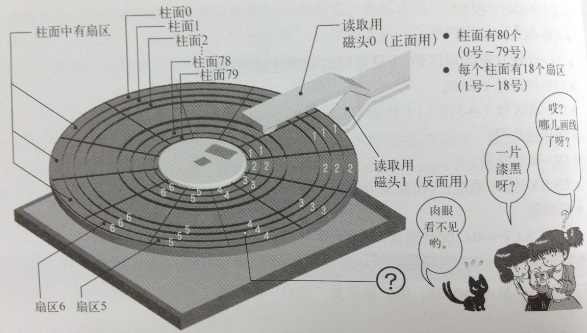
\includegraphics[width=0.6\textwidth]{day03-ruanpan.jpg}\\
  \caption{软盘的结构}\label{ruanpan}
\end{figure}

一张软盘有80个柱面,2个磁头,18个扇区,且一个扇区有512字节。所以一张软盘的容量是$80\times 2\times 18\times 512=1474560 Byte= 1440KB$。

含有IPL的启动区,位于C0-H0-S1(柱面0,磁头0,扇区1),下一个扇区是C0-H0-S2,这次我们要装载的扇区就是这个。

ES:BX=缓冲地址~是个内存地址,表明要把软盘上读出的数据装载到内存的哪个位置。由于一个BX只能表示0$\sim$0xffff的值,即64K,太小了,使用段寄存器以ES:BX这种方式来表示地址,写成“MOV AL,[ES:BX]”,代表“ES$\times$16+BX” 的内存地址。程序中指定了ES=0x0820,BX=0,所以软盘的数据会被装载到0x8200$\sim$0x83ff的位置。
\cs

作者使用变量的方式改写了Makefile文件,可以看一下。

\section{	试错	}
鉴于软盘的不可靠性,有时候需要在软盘读不出来的时候多读几次,这里重读5 次。

\dag|projects\03_day\harib00b|
\begin{code}[label=ipl.nas 本次添加的部分]
; ディスクを読む

		MOV		AX,0x0820
		MOV		ES,AX
		MOV		CH,0			; シリンダ0
		MOV		DH,0			; ヘッド0
		MOV		CL,2			; セクタ2

		MOV		SI,0			; 失敗回数を数えるレジスタ
retry:
		MOV		AH,0x02			; AH=0x02 : ディスク読み込み
		MOV		AL,1			; 1セクタ
		MOV		BX,0
		MOV		DL,0x00			; Aドライブ
		INT		0x13			; ディスクBIOS呼び出し
		JNC		fin				; エラーがおきなければfinへ
		ADD		SI,1			; SIに1を足す
		CMP		SI,5			; SIと5を比較
		JAE		error			; SI >= 5 だったらerrorへ
		MOV		AH,0x00
		MOV		DL,0x00			; Aドライブ
		INT		0x13			; ドライブのリセット
		JMP		retry
\end{code}

其中,JNC(jump if not carry),进位标志为0的话跳转;JAE(jump if above or equal),大于或等于时跳转。

在重新读盘之前,做了如下处理,AH=0x00,DL=0x00,INT=0x13,即完成系统复位。
\section{	读到18扇区	}
往后多读几个扇区,读完柱面0的18个扇区。

\dag|projects\03_day\harib00c|
\begin{code}[label=ipl.nas 本次添加的部分]
; ディスクを読む

		MOV		AX,0x0820
		MOV		ES,AX
		MOV		CH,0			; シリンダ0
		MOV		DH,0			; ヘッド0
		MOV		CL,2			; セクタ2
readloop:
		MOV		SI,0			; 失敗回数を数えるレジスタ
retry:
		MOV		AH,0x02			; AH=0x02 : ディスク読み込み
		MOV		AL,1			; 1セクタ
		MOV		BX,0
		MOV		DL,0x00			; Aドライブ
		INT		0x13			; ディスクBIOS呼び出し
		JNC		next			; エラーがおきなければnextへ
		ADD		SI,1			; SIに1を足す
		CMP		SI,5			; SIと5を比較
		JAE		error			; SI >= 5 だったらerrorへ
		MOV		AH,0x00
		MOV		DL,0x00			; Aドライブ
		INT		0x13			; ドライブのリセット
		JMP		retry
next:
		MOV		AX,ES			; アドレスを0x200進める
		ADD		AX,0x0020
		MOV		ES,AX			; ADD ES,0x020 という命令がないのでこうしている
		ADD		CL,1			; CLに1を足す
		CMP		CL,18			; CLと18を比較
		JBE		readloop		; CL <= 18 だったらreadloopへ
\end{code}

JBE(jump if below or equal),小于等于则跳转。

要读入下一个扇区只需给CL加1,给ES加上0x20(512/16)。CL是扇区号,ES指定读入地址。

这里使用循环的方式读入各个扇区,而不是在开始的时候设置读入的扇区数AL=17,因为磁盘BIOS读盘函数有一些“补充说明”:
\begin{quote}
  指定处理的扇区数,范围在0x01~0xff(指定0x02以上的数值时,要特别注意能够连续处理多个扇区的条件。如果是FD的话,似乎不能跨越多个磁道,也不能超过64KB的界限。)
\end{quote}

经过上面这些读盘处理,已经把磁盘上C0-H0-S2到C0-H0-S18的$512\times 17=8704$个字节的内容,装载到了内存的0x8200$\sim$0xa3ff。
\section{	读入10个柱面	}
C0-H0-S18扇区的下一个扇区是磁盘反面的C0-H1-S1,按顺序读到C0-H1-S18,接着读C1-H0-S1,最后一直读到C9-H1-S18。

\dag |projects\03_day\harib00d|
\begin{code}
; ディスクを読む

		MOV		AX,0x0820
		MOV		ES,AX
		MOV		CH,0			; シリンダ0
		MOV		DH,0			; ヘッド0
		MOV		CL,2			; セクタ2
readloop:
		MOV		SI,0			; 失敗回数を数えるレジスタ
retry:
		MOV		AH,0x02			; AH=0x02 : ディスク読み込み
		MOV		AL,1			; 1セクタ
		MOV		BX,0
		MOV		DL,0x00			; Aドライブ
		INT		0x13			; ディスクBIOS呼び出し
		JNC		next			; エラーがおきなければnextへ
		ADD		SI,1			; SIに1を足す
		CMP		SI,5			; SIと5を比較
		JAE		error			; SI >= 5 だったらerrorへ
		MOV		AH,0x00
		MOV		DL,0x00			; Aドライブ
		INT		0x13			; ドライブのリセット
		JMP		retry
next:
		MOV		AX,ES			; アドレスを0x200進める
		ADD		AX,0x0020
		MOV		ES,AX			; ADD ES,0x020 という命令がないのでこうしている
		ADD		CL,1			; CLに1を足す
		CMP		CL,18			; CLと18を比較
		JBE		readloop		; CL <= 18 だったらreadloopへ
		MOV		CL,1
		ADD		DH,1
		CMP		DH,2
		JB		readloop		; DH < 2 だったらreadloopへ
		MOV		DH,0
		ADD		CH,1
		CMP		CH,CYLS
		JB		readloop		; CH < CYLS だったらreadloopへ
\end{code}

JB(jump if below),如果小于就跳转。

在程序开头使用了EQU指令来声明常数,即|CYLS EQU 10|。
现在已经能够把软盘最初的$10\times 2\times 18\times512=184320 byte= 180KB $的内容完整的装载到内存中了。

\section{	着手开发操作系统	}
编写一个短小的程序,只让它HLT。

\dag |projects\03_day\harib00e|
\begin{code}[label=haribote.nas]
fin:
    HLT
    JMP fin
\end{code}

使用nask编译,输出成harbote.sys。用“make img”指令来生成映像文件。

使用作者最开始提到的二进制编辑器查看haribote.img 和haribote.sys内容,可以发现0x002600附近保存着文件名,0x004200位置保存着文件的内容,这里分别是haribotesys 和编译后的harbote.sys里面的内容“|F4 EB FD|”。

这样,要做的工作就是将操作系统的本身的内容写到名为harbote.sys的问卷中,再把它保存到磁盘映像里,然后从启动区执行这个harbote.sys 就行了。
\section{	从启动区执行操作系统	}
现在的程序是从启动区开始,把磁盘上的内容装载到内存 0x8000 号地址,所以磁盘映像上位于 0x004200 号地址的程序位于内存的0x8000+0x4200=0xc200号地址。

修改haribote.nas,加上ORG 0xc200,然后在ipl.nas处理的最后加上JMP 0xc200这个指令。详细程序见“projects/03\_day/harib00f”。

通过运行“make run”来运行程序。
\section{	确认操作系统的执行情况	}
通过切换以下画面模式,让画面变成一片漆黑,证明程序正常运行。

\dag |projects/03_day/harib00g|

\begin{code}
; haribote-os
; TAB=4

		ORG		0xc200			; このプログラムがどこに読み込まれるのか

		MOV		AL,0x13			; VGAグラフィックス、320x200x8bitカラー
		MOV		AH,0x00
		INT		0x10
fin:
		HLT
		JMP		fin
\end{code}

设置显卡模式:
\begin{itemize}
  \item AH=0x00
  \item AL=模式:
  \begin{itemize}
    \item 0x03:16色字符模式,80$\times$25
    \item 0x12:VGA图形模式,640$\times$480$\times$4位彩色模式,独特的4面存储模式
    \item 0x13:VGA图形模式,320$\times$200$\times$8位彩色模式,调色板模式
    \item 扩展VGA图形模式,800$\times$600$\times$4位彩色模式,独特的4面存储模式
  \end{itemize}
  \item 返回值:无
\end{itemize}

程序的变动:
将ipl.nas改名为ipl10.nas,提醒这个程序只能读入10个柱面。

想把磁盘装载内容的结束地址告诉给haribote.sys,在ipl10.nas文件中“JMP 0xc200”之前加入了一行代码,将CYLS的值写到内存地址0x0ff0中。

运行“make run”查看效果,应该是一片漆黑画面。

\section[32位模式前期准备]{32位模式前期准备\protect\footnote{书中作者先讲述了为什么用32位模式,自己看下书吧。}}

考虑到系统以后会支持各种不同的画面模式,就需要把现在的设置信息(BOOT\_INFO)保存起来以备后用。

\dag|projects\03_day\harib00h|
\begin{code}[label=haribote.nas]
; haribote-os
; TAB=4

; BOOT_INFO関係
CYLS	EQU		0x0ff0			; ブートセクタが設定する
LEDS	EQU		0x0ff1
VMODE	EQU		0x0ff2			; 色数に関する情報。何ビットカラーか?
SCRNX	EQU		0x0ff4			; 解像度のX
SCRNY	EQU		0x0ff6			; 解像度のY
VRAM	EQU		0x0ff8			; グラフィックバッファの開始番地

		ORG		0xc200			; このプログラムがどこに読み込まれるのか

		MOV		AL,0x13			; VGAグラフィックス、320x200x8bitカラー
		MOV		AH,0x00
		INT		0x10
		MOV		BYTE [VMODE],8	; 画面モードをメモする
		MOV		WORD [SCRNX],320
		MOV		WORD [SCRNY],200
		MOV		DWORD [VRAM],0x000a0000

; キーボードのLED状態をBIOSに教えてもらう

		MOV		AH,0x02
		INT		0x16 			; keyboard BIOS
		MOV		[LEDS],AL

fin:
		HLT
		JMP		fin
\end{code}

|[VRAM]|里保存的是 0xa0000。VRAM是显卡内存,它的各个地址对应画面上的像素。不同的画面模式对应不同的VRAM,因此这里将使用的VRAM地址保存在BOOT\_INFO里。这种画面模式下VRAM是“0xa000$\sim$0xaffff的64KB”。画面的像素数、颜色数以及从BIOS取得的键盘信息都保存在内存0x0ff0位置附近。


\section{	开始导入C语言	}

现在,直接切换到32位模式,然后运行C语言写程序。

程序做了很大的改动,haribote.sys的前半部分使用汇编语言编写的,后半部分是用C语言编写的,所以将haribote.nas改成了asmhead.nas,并且,为了调用C 语言写的程序,添加了100行左右的汇编代码。这些汇编代码作者在后面再讲解,这里直接跳过,分析C语言部分。

C语言部分写在bootpack.c文件中。

\dag|projects\03_day\harib00i|
\begin{code}[label=bootpack.c]
void HariMain(void)
{

fin:
	/* ここにHLTを入れたいのだが、C言語ではHLTが使えない! */
	goto fin;

}
\end{code}

\cs

bootpack.c变成机器语言的过程:
\begin{enumerate}
  \item 使用ccl.exe从bootpack.c生成bootpack.gas;
  \item 使用gas2nask.exe从 bootpack.gas生成bootpack.nas;
  \item 使用nask.exe从bootpack.nas生成bootpack.obj;
  \item 使用obj2bim.exe从bootpack.obj生成bootpack.bim;
  \item 使用bim2hrb.exe从bootpack.bim生成bootpack.hrb;
  \item 使用copy指令将asmhead.bin与bootpack.hrb单纯结合起来就生成了haribote.sys。
\end{enumerate}

\section{	实现HLT(harib00j)	}

\dag|projects\03_day\harib00j|
\begin{code}[label=naskfun.nas]
; naskfunc
; TAB=4

[FORMAT "WCOFF"]				; オブジェクトファイルを作るモード	
[BITS 32]						; 32ビットモード用の機械語を作らせる


; オブジェクトファイルのための情報

[FILE "naskfunc.nas"]			; ソースファイル名情報

		GLOBAL	_io_hlt			; このプログラムに含まれる関数名


; 以下は実際の関数

[SECTION .text]		; オブジェクトファイルではこれを書いてからプログラムを書く

_io_hlt:	; void io_hlt(void);
		HLT
		RET
\end{code}

使用汇编语言编写了一个函数,io\_hlt。将输出设置为WCOFF模式,可以编译成目标文件,与bootpack.obj链接。

在nask目标文件的模式下,必须设定文件名信息,然后再写明下面程序的函数名。需要先在函数名前面加上“\_”,否则不能很好地与C语言函数链接。需要链接的函数名都需要GLOBAL指令声明。

下面写一个实际的函数。先写一个与用GLOBAL声明的函数名相同的标号,从此处开始写代码就可以了。

\dag|projects\03_day\harib00j|
\begin{code}[label=bootpack.c]
/* 他のファイルで作った関数がありますとCコンパイラに教える */

void io_hlt(void);

/* 関数宣言なのに、{}がなくていきなり;を書くと、
	他のファイルにあるからよろしくね、という意味になるのです。 */

void HariMain(void)
{

fin:
	io_hlt(); /* これでnaskfunc.nasの_io_hltが実行されます */
	goto fin;

}
\end{code}


“make run”运行程序。

%\chapter{	C语言与画面显示的练习	}
\section{	用C语言实现内存写入(harib01a)	}
在让画面黑屏的基础上,通过写VRAM的值,在画面上画出些“花”来。

\dag|projects\04_day\harib01a|
\begin{code}[label=naskfunc.nas]
_write_mem8:	; void write_mem8(int addr, int data);
		MOV		ECX,[ESP+4]		; [ESP+4]にaddrが入っているのでそれをECXに読み込む
		MOV		AL,[ESP+8]		; [ESP+8]にdataが入っているのでそれをALに読み込む
		MOV		[ECX],AL
		RET
\end{code}

C语言部分:
\begin{code}[label=bootpack.c]
void io_hlt(void);
void write_mem8(int addr, int data);

void HariMain(void)
{
	int i; /* 変数宣言。iという変数は、32ビットの整数型 */

	for (i = 0xa0000; i <= 0xaffff; i++) {
		write_mem8(i, 15); /* MOV BYTE [i],15 */
	}

	for (;;) {
		io_hlt();
	}
}
\end{code}

VRAM中都写入了15,意思是全部像素的颜色都是第15种颜色,即白色,因此运行程序后画面会变成白色。
\section{	条纹图案(harib01b)	}
\dag|projects\04_day\harib01b|
\begin{code}[label=bootpack.c]

	for (i = 0xa0000; i <= 0xaffff; i++) {
		write_mem8(i, i&0x0f); 
	}
\end{code}

通过与运算,将15改成特殊的值,低4位保持不变,高4位全部变成0。这样每隔16个像素,色号就反复一次。


\section{	挑战指针(harib01c)	}
使用C语言的指针,修改上面程序,实现内存写入。

\dag|projects\04_day\harib01c|
\begin{code}
void io_hlt(void);

void HariMain(void)
{
	int i; /* 変数宣言。iという変数は、32ビットの整数型 */
	char *p; /* pという変数は、BYTE [...]用の番地 */

	for (i = 0xa0000; i <= 0xaffff; i++) {

		p = i; /* 番地を代入 */
		*p = i & 0x0f;

		/* これで write_mem8(i, i & 0x0f); の代わりになる */
	}

	for (;;) {
		io_hlt();
	}
}
\end{code}
\section{	指针的应用(1)(harib01d)	}
\section{	指针的应用(2)(harib01e)	}
\section{	色号设定(harib01f)	}
\section{	绘制矩形(harib01g)	}
\section{	今天的成果(harib01h)	}


%\chapter{	结构体、文字显示与GDT/IDT初始化	}
\section{	接收启动信息(harib02a)	}
\section{	试用结构体(harib02b)	}
\section{	试用箭头记号(harib02c)	}
\section{	显示字符(harib02d)	}
\section{	增加字体(harib02e)	}
\section{	显示字符串(harib02f)	}
\section{	显示变量值(harib02g)	}
\section{	显示鼠标指针(harib02h)	}
\section{	GDT与IDT的初始化(harib02i)	}


%\chapter{	分割编译与中断处理	}
\section{	分割源文件(harib03a)	}
将bootpack.c分割成了graphic.c、dsctbl.c、bootpack.c。
\section{	整理Makefile(harib03b)	}
将处理相同事情的部分归纳,按照一般规则来处理。
\section{	整理头文件(harib03c)	}
将各个源文件重复部分去掉,归纳起来,放到bootpack.h的头文件里。在具体的源文件里引用头文件。
\section{	意犹未尽	}
介绍上一章naskfunc.nas的|load_gdtr|函数:
\begin{code}
_load_gdtr:		; void load_gdtr(int limit, int addr);
		MOV		AX,[ESP+4]		; limit
		MOV		[ESP+6],AX
		LGDT	[ESP+6]
		RET
\end{code}
函数用来将指定的段上限(limit)和地址赋值给名为GDTR的48位寄存器。这是一个很特别的48位寄存器,并不能用我们常用的MOV指令来赋值。给它赋值的时候,唯一的方法就是指定内存地址,从指定的地址读取6个字节,然后复制给GDTR寄存器。完成这一任务的就是LGDT。

该寄存器的低16位是段上限,它等于“GDT的有效字节数-1”。剩下的高32位代表GDT的开始地址。

在最初执行这个函数的时候,|DWORD[ESP+4]|里存放的是段上限,|DWORD[ESP+8]|里存放的是地址。具体到实际的数值,就是0x000fff和0x00270000。把它们按字节写出来的话就成了|FF FF 00 00 00 27 00|(注意地位放在内存地址小的字节里)。为了执行LGDT,希望把它们排列成|FF FF 00 00 00 27 00|的样子,所以就先用“|MOV AX,[ESP+4]|”读取最初的0xffff,然后再写到|[ESP+6]|里。这样结果就成了|[FF FF FF FF 00 27 00 00]|,如果从|[ESP+6]|开始读6字节的话,正好是我们想要的结果。

书中补充了dsctbl.c里的|set_segmdesc|函数及相关段的知识。具体内容参见书本。
\section{	初始化PIC(harib03d)	}
为了达到鼠标指针移动的目的,必须使用中断,而要使用中断必须将GDT和IDT正确无误的初始化。此时,需要初始化PIC。

PIC(programmable interrupt controller),可编程中断控制器。PIC将8个中断信号(IRQ)集合成一个中断信号的装置。PIC监视输入管脚的8 个中断信号,只要有一个中断信号进来,就将唯一的输出管脚信号变成ON,并通知给CPU。最初设计者希望通过增加PIC来处理更多的中断信号,把中断信号设计成15 个,增设了2个PIC(主从PIC)。

\cs

\dag|projects\06_day\harib03d|
\begin{code}[label=int.c的主要组成部分]
void init_pic(void)
/* PICの初期化 */
{
	io_out8(PIC0_IMR,  0xff  ); /* 全ての割り込みを受け付けない */
	io_out8(PIC1_IMR,  0xff  ); /* 全ての割り込みを受け付けない */

	io_out8(PIC0_ICW1, 0x11  ); /* エッジトリガモード */
	io_out8(PIC0_ICW2, 0x20  ); /* IRQ0-7は、INT20-27で受ける */
	io_out8(PIC0_ICW3, 1 << 2); /* PIC1はIRQ2にて接続 */
	io_out8(PIC0_ICW4, 0x01  ); /* ノンバッファモード */

	io_out8(PIC1_ICW1, 0x11  ); /* エッジトリガモード */
	io_out8(PIC1_ICW2, 0x28  ); /* IRQ8-15は、INT28-2fで受ける */
	io_out8(PIC1_ICW3, 2     ); /* PIC1はIRQ2にて接続 */
	io_out8(PIC1_ICW4, 0x01  ); /* ノンバッファモード */

	io_out8(PIC0_IMR,  0xfb  ); /* 11111011 PIC1以外は全て禁止 */
	io_out8(PIC1_IMR,  0xff  ); /* 11111111 全ての割り込みを受け付けない */

	return;
}
\end{code}

以上是PIC的初始化程序。从CPU的角度看,PIC是外部设备,CPU使用OUT指令进行操作,程序中的PIC0和PIC1,分别指主PIC和从PIC。PIC内部有很多寄存器,用端口号码对彼此进行区别,以决定是写入哪一个寄存器。具体的端口号码写在bootpack.h里。

\cs

PIC寄存器是8位寄存器。IMR(interrupt mask register)是中断屏蔽寄存器。8位分别对应8路IRQ信号。如果某一位的值是1,则该位所对应的IRQ信号被屏蔽,PIC就忽略该路信号。这主要是因为,正在对中断设定进行更改时,如果再接受别的中断信号会引起混乱,为了防止这种情况发生,就必须屏蔽中断。还有,如果某个IRQ没有连接任何设备的话,静电干扰也可能会引起反应,导致操作系统混乱,所以也要屏蔽掉这类干扰。

ICW(initial control word)是初始化控制数据。ICW有4个,分别编号为1$\sim$4,共有4个字节的数据。ICW1和ICW4主板配线方式、中断信号的电气特性等有关,不再叙述。ICW3是有关主-从连接的设定,对主PIC而言,第几号IRQ与从PIC相连,是用8位来设定的。对从PIC而言,该PIC与主PIC的第几号相连是用3位来设定。

\cs

不同的操作系统可以进行独特设定的只有ICW2。它决定了IRQ以哪一个信号中断通知CPU。

这次是以|INT 0x20~0x2f|接收中断信号IRQ0$\sim$15而设定的,因为INT 0x00$\sim$0x1f用于应用程序想对操作系统干坏事的时候CPU内部系统保护通知,所以直接使用|INT 0x20~0x2f|。

\section[中断处理程序的制作(harib03e)]{中断处理程序的制作(harib03e)\protect\footnote{书中讲到了IRQ1和IRQ12的中断处理程序,光盘里面补充了IRQ7的中断处理程序。详细解释见书。}}
鼠标是IRQ12,键盘是IRQ1,编写了用于INT 0x2c和INT 0x21的中断处理程序(handler),即中断发生时要调用的程序。

\begin{code}[label=int.c节选]
void inthandler21(int *esp)
/* PS/2キーボードからの割り込み */
{
	struct BOOTINFO *binfo = (struct BOOTINFO *) ADR_BOOTINFO;
	boxfill8(binfo->vram, binfo->scrnx, COL8_000000, 0, 0, 32 * 8 - 1, 15);
	putfonts8_asc(binfo->vram, binfo->scrnx, 0, 0, COL8_FFFFFF, "INT 21 (IRQ-1) : PS/2 keyboard");
	for (;;) {
		io_hlt();
	}
}
\end{code}
程序只是显示一条信息,然后保持在待机状态。鼠标的程序也几乎完全相同。

\cs

中断执行后不能执行return,而是必须执行IRETD指令。借助汇编语言修改naskfunc.nas。

\dag|projects\06_day\harib03e|
\begin{code}[label=naskfunc.nas节选]
		EXTERN	_inthandler21, _inthandler27, _inthandler2c

_asm_inthandler21:
		PUSH	ES
		PUSH	DS
		PUSHAD
		MOV		EAX,ESP
		PUSH	EAX
		MOV		AX,SS
		MOV		DS,AX
		MOV		ES,AX
		CALL	_inthandler21
		POP		EAX
		POPAD
		POP		DS
		POP		ES
		IRETD
\end{code}

其中,PUSHAD 相当于:
\begin{code}
PUSH EAX
PUSH ECX
PUSH EDX
PUSH EBX
PUSH ESP
PUSH EBP
PUSH ESI
PUSH EDI
\end{code}
POPAD相当于按以上相反的顺序,把它们全都POP出来。

\cs

函数只是将寄存器的值保存到栈里,然后将DS和ES调整到与SS相等,再调用\_inthandler21,返回以后,将所有寄存器的值再返回到原来的值,然后执行IRETD。

\cs

将这个函数注册到IDT中去,在dsctbl.c的|init_gdtidt|里加入以下语句。

\begin{code}
    /* IDTの設定 */
	set_gatedesc(idt + 0x21, (int) asm_inthandler21, 2 * 8, AR_INTGATE32);
	set_gatedesc(idt + 0x27, (int) asm_inthandler27, 2 * 8, AR_INTGATE32);
	set_gatedesc(idt + 0x2c, (int) asm_inthandler2c, 2 * 8, AR_INTGATE32);
\end{code}
|asm_inthandler21|注册在idt的第0x21号。这里的2$\times$8表示的是|asm_inthandler21|属于哪一个段,即段号是2,乘以8是因为低三位有别的意思,这里低三位必须为0,相当于写成“2<<3”。

号码为2的段,正好涵盖了整个bootpack.hrb。最后的|AR_CODE32_ER|将IDT的属性设定为0x008e。它表示这是用于中断处理的有效设定。
\begin{code}
set_segmdesc(gdt + 2, LIMIT_BOTPAK, ADR_BOTPAK, AR_CODE32_ER);
\end{code}

\cs

对bootpack.c的Harimain的补充。“|io_sti();|”仅仅是执行STI指令,它是CLI的逆指令。在HariMain的最后,修改了PIC的IMR,以便接收来自键盘和鼠标的中断。

\cs

运行程序会发现,键盘的中断响应正常,鼠标的却不行。











%\chapter{	FIFO与鼠标控制	}
\section{	获取按键编码(harib04a)	}
现在,只要在键盘上按一按键,就会在屏幕上显示信息,其他的我们什么也做不了。我们将程序改善一下,让程序在按下一个键后不会结束,而是把按键的编码在画面上显示出来,这样就可以切实完成中断处理程序了。

更改的程序是init.c程序中的inthandler21函数,具体如下:
\begin{code}
#define PORT_KEYDAT		0x0060

void inthandler21(int *esp)
{
	struct BOOTINFO *binfo = (struct BOOTINFO *) ADR_BOOTINFO;
	unsigned char data, s[4];
	io_out8(PIC0_OCW2, 0x61);	/* IRQ-01受付完了をPICに通知 */
	data = io_in8(PORT_KEYDAT);

	sprintf(s, "%02X", data);
	boxfill8(binfo->vram, binfo->scrnx, COL8_008484, 0, 16, 15, 31);
	putfonts8_asc(binfo->vram, binfo->scrnx, 0, 16, COL8_FFFFFF, s);

	return;
}
\end{code}

\cs

程序中|io_out8(PIC0_OCW2, 0x61);|这句话用来通知PIC已经知道发生了IRQ1 中断。如果是IRQ3,则写成0x63。执行这句话之后,PIC继续时刻监视IRQ1中断是否发生,反过来,如果忘记了执行这句话,PIC就不再监视IRQ1中断,不管下次由键盘输入什么信息,系统都感知不到了。

\cs
程序所完成的,是将接收到的按键编码显示在画面上,然后结束中断处理。

\section{	加快中断处理(harib04b)	}
程序里有一个问题,那就是字符显示的内容被放在了中断处理程序中。

所谓中断处理,基本上就是打断CPU本来的工作,加塞要求进行处理,所以必须完成得干净利索。而且中断处理进行期间,不再接收别的中断。所以如果我们处理键盘的中断速度太慢,就会出现鼠标的运动不连贯、不能从网上接收数据等情况。

另一方面,字符显示要花大块的时间来进行处理。仅仅画一个字符,就要执行8 $\times$16=128次if语句,来判断是否要往VRAM里描画该像素。如果判定为描画该像素,还要执行内存写入指令。而且为确定具体往内存的哪个地方写,还要做很多地址计算。这些事情,在我们看来,或许只是一瞬间的事情,但在计算机看来,可不是这样。

谁也不知道其他中断会在哪个瞬间到来。事实上,很可能在键盘输入的同时,就有数据正在从网上下载,而PIC在等待键盘中断处理的结束。

\cs

解决方案是先将按键的编码接收下来,保存到变量里去,然后由HariMain偶尔去看看这个变量。如果发现有了数据,就把它显示出来。

\begin{code}
struct KEYBUF keybuf;

void inthandler21(int *esp)
{
	unsigned char data;
	io_out8(PIC0_OCW2, 0x61);	/* IRQ-01受付完了をPICに通知 */
	data = io_in8(PORT_KEYDAT);
	if (keybuf.flag == 0) {
		keybuf.data = data;
		keybuf.flag = 1;
	}
	return;
}
\end{code}

考虑到键盘的输入时需要缓冲区,先定义一个构造体,命名为keybuf。 其中的flag变量用于表示这个缓冲区是否为空。如果flag是0,表示缓冲区为空;如果flag为1,表示缓冲区中有数据。那么,如果缓冲区有数据,而这时又来了一个中断,那么该怎么办呢?先不管哈~

\cs

\begin{code}[label=bootpack.c中HariMain函数节选]
for (;;) {
		io_cli();
		if (keybuf.flag == 0) {
			io_stihlt();
		} else {
			i = keybuf.data;
			keybuf.flag = 0;
			io_sti();
			sprintf(s, "%02X", i);
			boxfill8(binfo->vram, binfo->scrnx, COL8_008484, 0, 16, 15, 31);
			putfonts8_asc(binfo->vram, binfo->scrnx, 0, 16, COL8_FFFFFF, s);
		}
	}
\end{code}

开始先用|io_cli|指令屏蔽中断。

如果flag的值是0,说明键还没有被按下,keybuf.data里没有值 保存下来。在keybuf.data里有值被保存下来之前我们无事可做,所以干脆去执行|io_hlt|。但是,由于已经执行了|io_cli|屏蔽了中断,如果这样就去执行HLT指令的话,即使没有什么键被按下,程序也不会有任何反应。所以STI和HLT都要执行,而执行这两个指令的函数就是|io_stihlt|。执行HLT指令以后,如果收到了PIC的通知,CPU就会被唤醒。这样,CPU首先会去执行中断处理程序。中断处理程序执行完之后,又回到for语句的开头,再执行|io_cli|函数。

如果通过中断处理函数在keybuf.data里存入了按键编码,else语句就会被执行。先将这个键码(keybuf.data)值保存到变量i里,然后将flag 置为0表示键码值清为空,最后再通过|io_sti|语句开放中断。

\cs

运行程序,能够顺利执行……但是,右Ctrl键的显示是有问题的。

查阅资料得知,当按下右Ctrl键时,会产生两个字节的键码值“E0 1D”,而松开这个键之后,会产生两个字节的键码值“E0 9D”。在一次产生两个字节键码值的情况下,因为键盘内部电路一次只能发送一个字节,所以一次按键会产生两次中断,第一次中断时发送E0,第二次中断发生1D。

在harib04a中,以上两次中断所发送的值都能收到,瞬间显示E0后,紧接着又显示1D或者9D。而在harib04b中,HariMain函数在收到E0之前,又收到前一次按键产生的1D或者9D,而这个字节被舍弃了。

\section{	制作FIFO缓冲区(harib04c)	}
问题在于这里创建的缓冲区只存储一个字节,如果做一个能够存储多字节的缓冲区,那么它就不会满,问题也就解决了。

根据这种思路,有一下程序:
\begin{code}
struct KEYBUF {
	unsigned char data[32];
	int next;
};

void inthandler21(int *esp)
{
	unsigned char data;
	io_out8(PIC0_OCW2, 0x61);	/* IRQ-01受付完了をPICに通知 */
	data = io_in8(PORT_KEYDAT);
	if (keybuf.next < 32) {
		keybuf.data[keybuf.next] = data;
		keybuf.next++;
	}
	return;
}
\end{code}

keybuf.next的起点是“0”,所以最初存储的数据是keybuf.data[0],共32个存储位置。

下一个存储位置用变量next来管理。这样就可以记住32个数据,而不会溢出,但是为保险起见,next的值变成32之后,就舍去不要了。

\cs

取得数据的程序如下:

\begin{code}
	for (;;) {
		io_cli();
		if (keybuf.next == 0) {
			io_stihlt();
		} else {
			i = keybuf.data[0];
			keybuf.next--;
			for (j = 0; j < keybuf.next; j++) {
				keybuf.data[j] = keybuf.data[j + 1];
			}
			io_sti();
			sprintf(s, "%02X", i);
			boxfill8(binfo->vram, binfo->scrnx, COL8_008484, 0, 16, 15, 31);
			putfonts8_asc(binfo->vram, binfo->scrnx, 0, 16, COL8_FFFFFF, s);
		}
	}
\end{code}

如果next不是0,则说明至少有一个数据。最开始的一个数据肯定是放在|data[0]|中的,将这个数据存入到变量i中去。这样,数就减少一个,所以将next减去1。

接下来,for循环中,数据的存放位置全部都向前移送一个位置。

\cs
此时,右Ctrl的处理运行正常。但从|data[0]|取得数据后有关数据移送的处理不尽如人意。

数据移送处理本身没有什么不好,只是在禁止中断期间做数据移送处理有问题。但如果在数据移送处理前就允许中断的话,会搞乱要处理的数据,这当然不行。下面解决。
\section{	改善FIFO缓冲区(harib04d)	}
想开发一个不需要数据移送操作的FIFO型缓冲区。基本思路是:不仅维护下一个要写入数据的位置,还要维护下一个要读出数据的位置。这就像数据读出位置在追着数据写入位置跑一样。这样就不需要数据移送操作了。数据读出位置追上数据写入位置的时候,就相当于缓冲区为空,没有数据。

但是这样的缓冲区使用一段时间后,下一个数据写入位置会变成31,而这时下一个数据读出位置可能已经是29或30什么的了。当下一个写入位置变成32的时候,就走到死胡同了。因为下面没地方可以写入数据了。

如果当下一个数据写入位置到达缓冲区终点时,数据读出位置也恰好到达缓冲区终点,也就是说缓冲区正好变空,那还好说。我们只要将下一个数据写入位置和下一个数据读出位置都再置为0就行了,就像转回去从头再来一样。

但是总还是会有数据读出位置没有追上数据写入位置的情况。这时,又不得不进行数据移送操作。原来是每次都要进行数据移送,而现在不用每次都做。

仔细想一下,当下一个数据写入位置到达缓冲区最末尾,缓冲区开头部分应该已经变空了(如果还没有变空,说明数据读出跟不上数据写入,只能把部分数据扔掉了)。因此如果下一个数据写入位置到了32以后,就强制性地将它设置为0.这样一来,下一个数据写入位置就跑到了下一个数据读出位置的后面,让人觉得怪怪的。但这无关紧要,没什么问题。

对下一个数据读出位置也做同样的处理,一旦到了32以后,就把它设置为从0开始继续读取数据。这样32字节的缓冲区就能一圈一圈地不停循环,长久使用。数据移送操作一次都不需要。

\cs

相应的代码如下:
\begin{code}[label=bootpack.h节选]
struct KEYBUF {
	unsigned char data[32];
	int next_r, next_w, len;
};
\end{code}

变量len是指缓冲区能记录多少字节的数据。

\begin{code}[label=int.c节选]
void inthandler21(int *esp)
{
	unsigned char data;
	io_out8(PIC0_OCW2, 0x61);	/* IRQ-01受付完了をPICに通知 */
	data = io_in8(PORT_KEYDAT);
	if (keybuf.len < 32) {
		keybuf.data[keybuf.next_w] = data;
		keybuf.len++;
		keybuf.next_w++;
		if (keybuf.next_w == 32) {
			keybuf.next_w = 0;
		}
	}
	return;
}
\end{code}

读出数据程序如下:
\begin{code}
	for (;;) {
		io_cli();
		if (keybuf.len == 0) {
			io_stihlt();
		} else {
			i = keybuf.data[keybuf.next_r];
			keybuf.len--;
			keybuf.next_r++;
			if (keybuf.next_r == 32) {
				keybuf.next_r = 0;
			}
			io_sti();
			sprintf(s, "%02X", i);
			boxfill8(binfo->vram, binfo->scrnx, COL8_008484, 0, 16, 15, 31);
			putfonts8_asc(binfo->vram, binfo->scrnx, 0, 16, COL8_FFFFFF, s);
		}
	}
\end{code}
\section{	整理FIFO缓冲区(harib04e)	}
将结构做成这样:
\begin{code}
struct FIFO8 {
	unsigned char *buf;
	int p, q, size, free, flags;
};
\end{code}

如果我们将缓冲区大小固定成32字节的话,以后改起来就不方便了,所以把它定义成可变的。缓冲区的总字节数保存在变量size里。变量free 用于保存缓冲区里没有数据的字节数。缓冲区地址保存在变量buf里。p 代表下一个数据写入地址,q代表下一个数据读出地址。
\begin{code}
void fifo8_init(struct FIFO8 *fifo, int size, unsigned char *buf)
/* FIFOバッファの初期化 */
{
	fifo->size = size;
	fifo->buf = buf;
	fifo->free = size; /* 空き */
	fifo->flags = 0;
	fifo->p = 0; /* 書き込み位置 */
	fifo->q = 0; /* 読み込み位置 */
	return;
}
\end{code}

|fifo8_init|是结构的初始化函数,用来设定各种初始值,也就是设定FIFO8结构的地址以及与结构有关的各种参数。

\begin{code}
#define FLAGS_OVERRUN		0x0001

int fifo8_put(struct FIFO8 *fifo, unsigned char data)
/* FIFOへデータを送り込んで蓄える */
{
	if (fifo->free == 0) {
		/* 空きがなくてあふれた */
		fifo->flags |= FLAGS_OVERRUN;
		return -1;
	}
	fifo->buf[fifo->p] = data;
	fifo->p++;
	if (fifo->p == fifo->size) {
		fifo->p = 0;
	}
	fifo->free--;
	return 0;
}
\end{code}

|fifo8_put|是往FIFO缓冲区存储1字节信息的函数。用flags这一变量来记录是否溢出。

\begin{code}
int fifo8_get(struct FIFO8 *fifo)
/* FIFOからデータを一つとってくる */
{
	int data;
	if (fifo->free == fifo->size) {
		/* バッファが空っぽのときは、とりあえず-1が返される */
		return -1;
	}
	data = fifo->buf[fifo->q];
	fifo->q++;
	if (fifo->q == fifo->size) {
		fifo->q = 0;
	}
	fifo->free++;
	return data;
}
\end{code}

|fifo8_get|是从FIFO缓冲区取出1字节的函数。
\begin{code}
int fifo8_status(struct FIFO8 *fifo)
/* どのくらいデータが溜まっているかを報告する */
{
	return fifo->size - fifo->free;
}
\end{code}

|fifo8_status|用来查看缓冲区状态。

使用以上函数,写成的程序段如下:
\begin{code}
struct FIFO8 keyfifo;

void inthandler21(int *esp)
{
	unsigned char data;
	io_out8(PIC0_OCW2, 0x61);	/* IRQ-01受付完了をPICに通知 */
	data = io_in8(PORT_KEYDAT);
	fifo8_put(&keyfifo, data);
	return;
}
\end{code}

MariMain函数内容如下:
\begin{code}
	char s[40], mcursor[256], keybuf[32];

	fifo8_init(&keyfifo, 32, keybuf);

	for (;;) {
		io_cli();
		if (fifo8_status(&keyfifo) == 0) {
			io_stihlt();
		} else {
			i = fifo8_get(&keyfifo);
			io_sti();
			sprintf(s, "%02X", i);
			boxfill8(binfo->vram, binfo->scrnx, COL8_008484, 0, 16, 15, 31);
			putfonts8_asc(binfo->vram, binfo->scrnx, 0, 16, COL8_FFFFFF, s);
		}
	}
\end{code}

程序运行正常!
\section{	总算讲到鼠标了(harib04f)	}
较计算机的历史来说,鼠标比较新,早起的计算机并不支持,这一点从鼠标的中段号码IRQ12这一很大的数字就可以看出。

鼠标作为计算机的一个外部设备开始使用的时候,几乎所有的操作系统都不支持它。在这种情况下,如果只是稍微一动鼠标就产生中断的话,那么使用那些操作系统的时候,就只好把鼠标先拔掉。这是很不方便的。为了不影响鼠标和其它设备的使用,主板上做了鼠标用的电路,但是只要不执行激活鼠标的指令,就不产生鼠标的中断信号。

所谓不产生中断信号,也就是说,即使从鼠标传来了数据,CPU也不会接收。这样的话鼠标也就没必要传送数据了,否则会引起电路的混乱。所以,处于初期状态的鼠标,不管是滑动操作还是点击操作,都没有反应。

总而言之,我们必须发现指令,让下面两个装置有效,一个是鼠标控制电路,一个是鼠标本身。

\cs

控制电路的设定。事实上,鼠标控制电路包含着键盘控制电路里,如果键盘控制电路的初始化正常完成,鼠标电路控制器的激活也就完成了。

\begin{code}
#define PORT_KEYDAT				0x0060
#define PORT_KEYSTA				0x0064
#define PORT_KEYCMD				0x0064
#define KEYSTA_SEND_NOTREADY	0x02
#define KEYCMD_WRITE_MODE		0x60
#define KBC_MODE				0x47

void wait_KBC_sendready(void)
{
	/* キーボードコントローラがデータ送信可能になるのを待つ */
	for (;;) {
		if ((io_in8(PORT_KEYSTA) & KEYSTA_SEND_NOTREADY) == 0) {
			break;
		}
	}
	return;
}

void init_keyboard(void)
{
	/* キーボードコントローラの初期化 */
	wait_KBC_sendready();
	io_out8(PORT_KEYCMD, KEYCMD_WRITE_MODE);
	wait_KBC_sendready();
	io_out8(PORT_KEYDAT, KBC_MODE);
	return;
}
\end{code}

函数|wait_KBC_sendready|的作用是让键盘控制电路做好准备动作,等待控制指令的到来。是因为虽然CPU的电路很快,但键盘控制电路却没有那么快。如果CPU不顾设备接收数据的能力,只是一个劲儿地发指令的话,有些指令会得不到执行,从而导致错误的结果。如果键盘控制电路可以接受CPU指令了,CPU从设备号码0x0064处所读取的数据的倒数第二位(从低位开始数的第二位)应该是0。在确认到这一位是0 之前,程序一直通过for语句循环查询。

|init_keyboard|一边确认可否往键盘控制电路传送信息,一边发送模式设定指令,指令中包含着要设定为何种模式。模式设定的指令是0x60,利用鼠标模式的模式号码是0x47。

在HariMain函数调用|init_keyboard|函数,鼠标控制电路的准备就完成了。

\cs

开始发送激活鼠标的指令。所谓发送鼠标激活指令,归根到底还是要向键盘控制器发送指令。
\begin{code}
#define KEYCMD_SENDTO_MOUSE		0xd4
#define MOUSECMD_ENABLE			0xf4

void enable_mouse(void)
{
	/* マウス有効 */
	wait_KBC_sendready();
	io_out8(PORT_KEYCMD, KEYCMD_SENDTO_MOUSE);
	wait_KBC_sendready();
	io_out8(PORT_KEYDAT, MOUSECMD_ENABLE);
	return; /* うまくいくとACK(0xfa)が送信されてくる */
}
\end{code}

往键盘控制电路发送指令0xd4,下一个数据就会自动发送给鼠标。激活的鼠标发送返回值oxfa。

在HariMain中调用函数,运行程序,鼠标中断可用。

\section{	从鼠标接受数据(harib04g)	}

取出中断数据:
\begin{code}
struct FIFO8 mousefifo;

void inthandler2c(int *esp)
/* PS/2マウスからの割り込み */
{
	unsigned char data;
	io_out8(PIC1_OCW2, 0x64);	/* IRQ-12受付完了をPIC1に通知 */
	io_out8(PIC0_OCW2, 0x62);	/* IRQ-02受付完了をPIC0に通知 */
	data = io_in8(PORT_KEYDAT);
	fifo8_put(&mousefifo, data);
	return;
}
\end{code}

IRQ-12是从PIC的第4号(从PIC相当于IRQ-08~IRQ-15),首先要通知IRQ-12受理已完成,然后再通知主PIC。这是因为主/从PIC的协调不能够自动完成,如果程序不教给主PIC该怎么做,它就会忽视从PIC的下一个中断请求。从PIC连接到主PIC的第2号上,这么做OK。

\cs

下面的鼠标数据取得方法,居然与键盘完全相同。靠中断号码来区分传到这个设备的数据究竟是来自键盘还是鼠标。

取得数据的程序如下:
\begin{code}
	fifo8_init(&mousefifo, 128, mousebuf);

	for (;;) {
		io_cli();
		if (fifo8_status(&keyfifo) + fifo8_status(&mousefifo) == 0) {
			io_stihlt();
		} else {
			if (fifo8_status(&keyfifo) != 0) {
				i = fifo8_get(&keyfifo);
				io_sti();
				sprintf(s, "%02X", i);
				boxfill8(binfo->vram, binfo->scrnx, COL8_008484,  0, 16, 15, 31);
				putfonts8_asc(binfo->vram, binfo->scrnx, 0, 16, COL8_FFFFFF, s);
			} else if (fifo8_status(&mousefifo) != 0) {
				i = fifo8_get(&mousefifo);
				io_sti();
				sprintf(s, "%02X", i);
				boxfill8(binfo->vram, binfo->scrnx, COL8_008484, 32, 16, 47, 31);
				putfonts8_asc(binfo->vram, binfo->scrnx, 32, 16, COL8_FFFFFF, s);
			}
		}
	}
\end{code}

因为鼠标往往会比键盘更快地送出大量数据,所以我们将它的FIFO缓冲区增加到了128字节。这样,就算是一下子来了很多数据,也不会溢出。

取得数据的程序中,如果键盘和鼠标的FIFO缓冲区都为空了,就执行HLT。如果不是两者都空,就先检查keyinfo,如果有数据,就取出一个显示出来。如果keyinfo是空,就再去检查mouseinfo,如果有数据,就取出一个显示出来。

程序运行正常。

%\chapter{	鼠标控制与32位模式切换	}
\section{	鼠标解读(1)(harib05a)	}
\section{	稍事整理(harib05b)	}
\section{	鼠标解读(2)(harib05c)	}
\section{	移动鼠标指针(harib05d)	}
\section{	通往32位模式之路	}


%\chapter{	内存管理	}
\section{	整理源文件(harib06a)	}
鼠标指针的叠加处理留待以后处理,先转向内存管理。

把bootpack.c里面的一些函数单独择出去。
\begin{table}[!ht]
  \centering
  \begin{tabular}{|l|l|l|}
  \hline
  % after \\: \hline or \cline{col1-col2} \cline{col3-col4} ...
  函数名 & 移动前 & 移动后 \\\hline
    wait\_KBC\_sendready&	bootpack.c&	keyboard.c\\
    init\_keyboard&	bootpack.c&	keyboard.c\\
    enable\_mouse&	bootpack.c&	mouse.c\\
    mouse\_decode&	bootpack.c&	mouse.c\\
    inthandler21&	init.c&	keyboard.c\\
    inthandler2c&	init.c&	mouse.c\\
    \hline
\end{tabular}
\end{table}

\section{	内存容量检查(1)(harib06b)	}

在进行内存管理之前,必须要做的事情是搞清楚内存究竟到底有多大,范围是到哪里。

在最初启动时,BIOS肯定要检查内存容量,所以只要我们问一问BIOS,就能知道内存容量有多大。但问题是,如果那样做的话,一方面asmhead.nas会变长,另一方面,BIOS版本不同,BIOS函数的调用方法也不相同,麻烦事太多了。所以,作者自己去检查内存。

内存检查时,要往内存里随便写入一个值,然后马上读取,来检查读取的值与写入的值是否相等。如果内存连接正常,则写入的值能够记在内存里。如果没连接上,则读出的值肯定是乱七八糟的。但是,如果CPU里加上了缓存会导致写入和读出的不是内存,而是缓存。结果,所有的内存都“正常”,检查处理不能完成。

所以,只有在内存检查时才将缓存设为OFF。具体来说,就是先查查CPU是不是在486以上,如果是,就将缓存设为OFF。按照这一思路,我们创建了以下函数memtest。

\begin{code}[label=bootpack.c节选]
#define EFLAGS_AC_BIT		0x00040000
#define CR0_CACHE_DISABLE	0x60000000

unsigned int memtest(unsigned int start, unsigned int end)
{
	char flg486 = 0;
	unsigned int eflg, cr0, i;

	/* 386か、486以降なのかの確認 */
	eflg = io_load_eflags();
	eflg |= EFLAGS_AC_BIT; /* AC-bit = 1 */
	io_store_eflags(eflg);
	eflg = io_load_eflags();
	if ((eflg & EFLAGS_AC_BIT) != 0) { /* 386ではAC=1にしても自動で0 に戻ってしまう */
		flg486 = 1;
	}
	eflg &= ~EFLAGS_AC_BIT; /* AC-bit = 0 */
	io_store_eflags(eflg);

	if (flg486 != 0) {
		cr0 = load_cr0();
		cr0 |= CR0_CACHE_DISABLE; /* キャッシュ禁止 */
		store_cr0(cr0);
	}

	i = memtest_sub(start, end);

	if (flg486 != 0) {
		cr0 = load_cr0();
		cr0 &= ~CR0_CACHE_DISABLE; /* キャッシュ許可 */
		store_cr0(cr0);
	}

	return i;
}
\end{code}

最初对EFLAGS进行的处理,是检查CPU是486以上还是386。如果是486以上,EFLAGS寄存器的第18位应该是所谓的AC标志位;如果CPU是386,那么就没有这个标志位,第18位一直是0。这里,我们有意识地把1写入到这一位,然后再读出EFLAGS的值,继而检查AC标志位是否仍为1。最后,将AC标志位重置为0。

将AC标志位重置为0时,用到了AND运算,那里出现了一个运算符“~”,它是取反运算符,就是将所有的位都反转的意思。所以,|~EFLAGS_AC_BIT|与0xfffbffff 一样。

为了禁止缓存,需要对CR0寄存器的某一标志位进行操作,需要用到函数|load_cr0| 和|store_cr0|,这个函数存在naskfunc.nas里。

\begin{code}[label=naskfunc.nas节选]
_load_cr0:		; int load_cr0(void);
		MOV		EAX,CR0
		RET

_store_cr0:		; void store_cr0(int cr0);
		MOV		EAX,[ESP+4]
		MOV		CR0,EAX
		RET
\end{code}

\cs

|memtest_sub|函数,是内存检查处理的实现部分。

\begin{code}
unsigned int memtest_sub(unsigned int start, unsigned int end)
{
	unsigned int i, *p, old, pat0 = 0xaa55aa55, pat1 = 0x55aa55aa;
	for (i = start; i <= end; i += 0x1000) {
		p = (unsigned int *) (i + 0xffc);
		old = *p;			/* いじる前の値を覚えておく */
		*p = pat0;			/* ためしに書いてみる */
		*p ^= 0xffffffff;	/* そしてそれを反転してみる */
		if (*p != pat1) {	/* 反転結果になったか? */
not_memory:
			*p = old;
			break;
		}
		*p ^= 0xffffffff;	/* もう一度反転してみる */
		if (*p != pat0) {	/* 元に戻ったか? */
			goto not_memory;
		}
		*p = old;			/* いじった値を元に戻す */
	}
	return i;
}
\end{code}

调查从start地址到end地址的范围内,能够使用的内存的末尾地址。首先如果p 不是指针,就不能指定地址去读取内存,所以先执行“p=i;”。紧接着使用这个p,将原值保存下来(变量old)。接着试写0xaa55aa55,在内存里反转该值,检查结果是否正确。如果正确,就再次反转它,检查一下是否能回复到初始值。最后,使用old变量,将内存的值恢复回去。如果在某个环节没能恢复成预想的值,那么就在那个环节终止调查,并报告终止时的地址。

for 语句中i 的增值部分以及p的赋值部分。每次只增加4,就要检查全部内存,速度太慢了,所以改成了每次增加0x1000,相当于4KB,这样一来速度就提高了1000倍。p的赋值计算式也变了,这是因为,如果不进行任何改变仍写作“p=i;”的话,程序就会只检查4KB最开头的4个字节。所以要改为“p=i + 0xffc;”,让它只检查末尾的4个字节。


\cs

修改HariMain程序,添加以下部分:
\begin{code}[label=bootpack.c节选]
	i = memtest(0x00400000, 0xbfffffff) / (1024 * 1024);
	sprintf(s, "memory %dMB", i);
	putfonts8_asc(binfo->vram, binfo->scrnx, 0, 32, COL8_FFFFFF, s);
\end{code}

暂时先使用以上程序对0x00400000~0xbfffffff范围的内存进行检查。这个程序最大可以识别3GB范围的内存。0x00400000号以前的内存已经被使用了(参考8.5节的内存分布图),没有内存,程序根本运行不到这里,所以我们没做内存检查。以MB为单位。

如果在QEMU上运行,根据模拟器的设定,内存应该为32MB。不过运行结果显示的是3072MB。有错误。

\section{	内存容量检查(2)(harib06c)	}

真正的原因是编译器对程序进行了优化,导致写的程序中有一些直接被「优化」掉了。

使用“make -r bootpack.nas”来运行的话,就可以确认bootpack.c被编译成了什么样的机器语言。用文本编辑器看一看生成的bootpack.nas会发现,最下边有|memtest_sub|的编译结果。

\begin{code}[label=memtest\_sub的编译结果]
_memtest_sub:
    PUSH    EBP                 ; C编译器的固定语句
    MOV EBP,ESP
    MOV EDX,DWORD [12+EBP]      ; EDX = end;
    MOV EAX,DWORD [8+EBP]       ; EAX = start; /* EAX是i */
    CMP EAX,EDX                 ; if (EAX > EDX) goto L30;
    JA  L30
L36:
L34:
    ADD EAX,4096                ; EAX += 0x1000;
    CMP EAX,EDX                 ; if (EAX <= EDX) goto L36;
    JBE L36
L30:
    POP EBP                     ; 接收前文中PUSH的EBP
    RET                         ; return;
\end{code}

与原始程序相比会发现,编译后没有XOR等指令,而且,好像编译后只剩下了for 语句。

\cs

编译器优化过程:

首先将内存的内容保存到old里,然后写入pat0的值,再反转,最后跟pat1进行比较。肯定相等,if语句不成立,得不到执行,所以把它删掉,将比较*p和pat0这部分也删掉。
\begin{code}
 unsigned int memtest_sub(unsigned int start, unsigned int end)
  {
      unsigned int i, *p, old, pat0 = 0xaa55aa55, pat1 = 0x55aa55aa;
      for (i = start; i <= end; i += 0x1000) {
          p = (unsigned int *) (i + 0xffc);

          old = *p;           /* 先记住修改前的值*/
          *p = pat0;          /* 试写 */
          *p ^= 0xffffffff;   /* 反转 */
          *p ^= 0xffffffff;   /* 再次反转 */
          *p = old;           /* 恢复为修改前的值 */
      }
      return i;
  }
\end{code}

反转了两次会变回之前的状态,所以这些处理也可以不要。
\begin{code}
unsigned int memtest_sub(unsigned int start, unsigned int end)
  {
      unsigned int i, *p, old, pat0 = 0xaa55aa55, pat1 = 0x55aa55aa;
      for (i = start; i <= end; i += 0x1000) {
          p = (unsigned int *) (i + 0xffc);
          old = *p;           /* 先记住修改前的值 */
          *p = pat0;          /* 试写 */
          *p = old;           /* 恢复为修改前的值 */
      }
      return i;
  }
\end{code}

还有,“*p = pat0;”本来就没有意义。反正要将old的值赋给*p。
\begin{code}
unsigned int memtest_sub(unsigned int start, unsigned int end)
  {
      unsigned int i, *p, old, pat0 = 0xaa55aa55, pat1 = 0x55aa55aa;
      for (i = start; i <= end; i += 0x1000) {
          p = (unsigned int *) (i + 0xffc);
          old = *p;           /* 先记住修改前的值 */
          *p = old;           /* 恢复为修改前的值 */
      }
      return i;
  }
\end{code}

*p里面实际没写进任何内容,删。
\begin{code}
unsigned int memtest_sub(unsigned int start, unsigned int end)
  {
      unsigned int i, *p, old, pat0 = 0xaa55aa55, pat1 = 0x55aa55aa;
      for (i = start; i <= end; i += 0x1000) {
          p = (unsigned int *) (i + 0xffc);
      }
      return i;
  }
\end{code}

这里的地址变量p,虽然计算了地址,却一次也没有用到,old、pat0、pat1 也都是用不到的变量。全部都舍弃掉。

\begin{code}
 unsigned int memtest_sub(unsigned int start, unsigned int end)
  {
      unsigned int i;
      for (i = start; i <= end; i += 0x1000) { }
      return i;
  }
\end{code}

根据以上编译器的思路,我们可以看出,它进行了最优化处理。但其实这个工作本来是不需要的。用于应用程序的C编译器,根本想不到会对没有内存的地方进行读写。

如果更改编译选项,是可以停止最优化处理的。可是在其他地方,我们还是需要如此考虑周密的最优化处理的,所以不想更改编译选项。于是决定|memtest_sub|也用汇编来写。

\begin{code}[label=naskfunc.nas节选]
_memtest_sub:   ; unsigned int memtest_sub(unsigned int start, unsigned int end)
		PUSH	EDI						; (EBX, ESI, EDI も使いたいので)
        PUSH    ESI
        PUSH    EBX
        MOV     ESI,0xaa55aa55          ; pat0 = 0xaa55aa55;
        MOV     EDI,0x55aa55aa          ; pat1 = 0x55aa55aa;
        MOV     EAX,[ESP+12+4]          ; i = start;
mts_loop:
        MOV     EBX,EAX
        ADD     EBX,0xffc               ; p = i + 0xffc;
        MOV     EDX,[EBX]               ; old = *p;
        MOV     [EBX],ESI               ; *p = pat0;
        XOR     DWORD [EBX],0xffffffff  ; *p ^= 0xffffffff;
        CMP     EDI,[EBX]               ; if (*p != pat1) goto fin;
        JNE     mts_fin
        XOR     DWORD [EBX],0xffffffff  ; *p ^= 0xffffffff;
        CMP     ESI,[EBX]               ; if (*p != pat0) goto fin;
        JNE     mts_fin
        MOV     [EBX],EDX               ; *p = old;
        ADD     EAX,0x1000              ; i += 0x1000;
        CMP     EAX,[ESP+12+8]          ; if (i <= end) goto mts_loop;

       JBE     mts_loop
        POP     EBX
        POP     ESI
        POP     EDI
        RET
mts_fin:
        MOV     [EBX],EDX               ; *p = old;
        POP     EBX
        POP     ESI
        POP     EDI
        RET
\end{code}

删除bootpack.c中的|memtest_sub|函数,运行程序。内存容量显示正常。
\section{	挑战内存管理(harib06d)	}
内存管理的基础,一是内存分配,一是内存释放。\footnote{建议找本操作系统的书看看各种内存管理方法。这里不想写了。}

内存管理程序:
\begin{code}[label=bootpack.c节选]
#define MEMMAN_FREES		4090	/* 偙傟偱栺32KB */

struct FREEINFO {	/* あき情報 */
	unsigned int addr, size;
};

struct MEMMAN {		/* メモリ管理 */
	int frees, maxfrees, lostsize, losts;
	struct FREEINFO free[MEMMAN_FREES];
};

void memman_init(struct MEMMAN *man)
{
	man->frees = 0;			/* あき情報の個数 */
	man->maxfrees = 0;		/* 状況観察用:freesの最大値 */
	man->lostsize = 0;		/* 解放に失敗した合計サイズ */
	man->losts = 0;			/* 解放に失敗した回数 */
	return;
}

unsigned int memman_total(struct MEMMAN *man)
/* あきサイズの合計を報告 */
{
	unsigned int i, t = 0;
	for (i = 0; i < man->frees; i++) {
		t += man->free[i].size;
	}
	return t;
}

unsigned int memman_alloc(struct MEMMAN *man, unsigned int size)
/* 確保 */
{
	unsigned int i, a;
	for (i = 0; i < man->frees; i++) {
		if (man->free[i].size >= size) {
			/* 十分な広さのあきを発見 */
			a = man->free[i].addr;
			man->free[i].addr += size;
			man->free[i].size -= size;
			if (man->free[i].size == 0) {
				/* free[i]がなくなったので前へつめる */
				man->frees--;
				for (; i < man->frees; i++) {
					man->free[i] = man->free[i + 1]; /* 構造体の代入 */
				}
			}
			return a;
		}
	}
	return 0; /* あきがない */
}
\end{code}

一开始的struct MEMMAN,创建了4000 组,留出不少余量,管理空间大约是32KB。其中还有变量 maxfrees、lostsize、losts等,这些变量与管理本身没有关系,不用在意它们。如果特别想了解的话,可以看看函数|memman_init|的注释,里面有介绍。

函数|memman_init|对memman进行了初始化,设定为空。主要工作,是将frees 设为0,而其他的都是附属性设定。

函数|memman_total|用来计算可用内存的合计大小并返回。

最后的|memman_alloc|函数,功能是分配指定大小的内存。除了|free[i].size| 变为0时的处理以外的部分,在前面已经说过了。

|memman_alloc|函数中|free[i].size|等于0的处理,与FIFO缓冲区的处理方法很相似,要进行移位处理。希望大家注意以下写法:
\begin{code}
man->free[i].addr = man->free[i+1].addr;

man->free[i].size = man->free[i+1].size;
\end{code}


我们在这里将其归纳为了:
\begin{code}
man->free[i] = man->free[i+1];
\end{code}

这种方法被称为结构体赋值,其使用方法如上所示,可以写成简单的形式。

\cs

释放内存函数,也就是往memman里追加可用内存信息的函数,稍微有点复杂。

\begin{code}[label=bootpack.c节选]
int memman_free(struct MEMMAN *man, unsigned int addr, unsigned int size)
/* 解放 */
{
	int i, j;
	/* まとめやすさを考えると、free[]がaddr順に並んでいるほうがいい */
	/* だからまず、どこに入れるべきかを決める */
	for (i = 0; i < man->frees; i++) {
		if (man->free[i].addr > addr) {
			break;
		}
	}
	/* free[i - 1].addr < addr < free[i].addr */
	if (i > 0) {
		/* 前がある */
		if (man->free[i - 1].addr + man->free[i - 1].size == addr) {
			/* 前のあき領域にまとめられる */
			man->free[i - 1].size += size;
			if (i < man->frees) {
				/* 後ろもある */
				if (addr + size == man->free[i].addr) {
					/* なんと後ろともまとめられる */
					man->free[i - 1].size += man->free[i].size;
					/* man->free[i]の削除 */
					/* free[i]がなくなったので前へつめる */
					man->frees--;
					for (; i < man->frees; i++) {
						man->free[i] = man->free[i + 1]; /* 構造体の代入 */
					}
				}
			}
			return 0; /* 成功終了 */
		}
	}
	/* 前とはまとめられなかった */
	if (i < man->frees) {
		/* 後ろがある */
		if (addr + size == man->free[i].addr) {
			/* 後ろとはまとめられる */
			man->free[i].addr = addr;
			man->free[i].size += size;
			return 0; /* 成功終了 */
		}
	}
	/* 前にも後ろにもまとめられない */
	if (man->frees < MEMMAN_FREES) {
		/* free[i]より後ろを、後ろへずらして、すきまを作る */
		for (j = man->frees; j > i; j--) {
			man->free[j] = man->free[j - 1];
		}
		man->frees++;
		if (man->maxfrees < man->frees) {
			man->maxfrees = man->frees; /* 最大値を更新 */
		}
		man->free[i].addr = addr;
		man->free[i].size = size;
		return 0; /* 成功終了 */
	}
	/* 後ろにずらせなかった */
	man->losts++;
	man->lostsize += size;
	return -1; /* 失敗終了 */
}
\end{code}

如果可用信息表满了,就按照舍去之后带来损失最小的原则进行割舍。但是在这个程序里,我们并没有对损失程度进行比较,而是舍去了刚刚进来的可用信息,这只是为了图个方便。

\cs

最后,将这个程序应用于HariMain,结果就变成了下面这样。

\begin{code}[label=bootpack.c节选]
#define MEMMAN_ADDR         0x003c0000

void HariMain(void)
{
    (中略)
    unsigned int memtotal;
    struct MEMMAN *memman = (struct MEMMAN *) MEMMAN_ADDR;
    (中略)
    memtotal = memtest(0x00400000, 0xbfffffff);
    memman_init(memman);
    memman_free(memman, 0x00001000, 0x0009e000); /* 0x00001000 - 0x0009efff */
    memman_free(memman, 0x00400000, memtotal - 0x00400000);
    (中略)
    sprintf(s, "memory %dMB   free : %dKB",
            memtotal / (1024 * 1024), memman_total(memman) / 1024);
    putfonts8_asc(binfo->vram, binfo->scrnx, 0, 32, COL8_FFFFFF, s);
\end{code}

memman需要32KB,我们暂时决定使用自0x003c0000开始的32KB(0x00300000号地址以后,今后的程序即使有所增加,预计也不会到达0x003c0000,所以我们使用这一数值),然后计算内存总量memtotal,将现在不用的内存以0x1000个字节为单位注册到memman里。最后,显示出合计可用内存容量。在QEMU上执行时,有时会注册成632KB和28MB。$632+28672=29304$,所以屏幕上会显示出29304KB。

 
%\chapter{	叠加处理	}
\section{	内存管理(续)(harib07a)	}
\section{	叠加处理(harib07b)	}
\section{	提高叠加处理速度(1)(harib07c)	}
\section{	提高叠加处理速度(2)(harib07d)	}


%\chapter{	制作窗口	}
\section{	鼠标显示问题(harib08a)	}
\section{	实现画面外的支持(harib08b)	}
\section{	shtctl的指定省略(harib08c)	}
\section{	显示窗口(harib08d)	}
\section{	小实验(harib08e)	}
\section{	高速计数器(harib08f)	}
\section{	消除闪烁(1)(harib08g)	}
\section{	消除闪烁(2)(harib08h)	}


%\chapter{	定时器(1)	}
\section{	使用定时器(harib09a)	}
\section{	计量时间(harib09b)	}
\section{	超时功能(harib09c)	}
\section{	设定多个定时器(harib09d)	}
\section{	加快中断处理(1)(harib09e)	}
\section{	加快中断处理(2)(harib09f)	}
\section{	加快中断处理(3)(harib09g)	}


%\chapter{	定时器(2)	}
\section{	简化字符串显示(harib10a)	}
\section{	重新调整FIFO缓冲区(1)(harib10b)	}
\section{	测试性能(harib10c~harib10f)	}
\section{	重新调整FIFO缓冲区(2)(harib10g)	}
\section{	加快中断处理(4)(harib10h)	}
\section{	使用“哨兵”简化程序(harib10i)	}


%\chapter{	高分辨率及键盘输入	}
\section{	继续测试性能(harib11a$\sim$harib11c)	}
\section{	提高分辨率(1)(harib11d)	}
\section{	提高分辨率(2)(harib11e)	}
\section{	键盘输入(1)(harib11f)	}
\section{	键盘输入(2)(harib11g)	}
\section{	追记内容(1)(harib11h)	}
\section{	追记内容(2)(harib11i)	}


%\chapter{	多任务(1)	}
\section{	挑战任务切换(harib12a)	}
\section{	任务切换进阶(harib12b)	}
\section{	做个简单的多任务(1)(harib12c)	}
\section{	做个简单的多任务(2)(harib12d)	}
\section{	提高运行速度(harib12e)	}
\section{	测试运行速度(harib12f)	}
\section{	多任务进阶(harib12g)	}


%\chapter{	多任务(2)	}
\section{	任务管理自动化(harib13a)	}
\section{	让任务休眠(harib13b)	}
\section{	增加窗口数量(harib13c)	}
\section{	设定任务优先级(1)(harib13d)	}
\section{	设定任务优先级(2)(harib13e)	}


%\chapter{	命令行窗口	}
\section{	闲置任务(harib14a)	}
\section{	创建命令行窗口(harib14b)	}
\section{	切换输入窗口(harib14c)	}
\section{	实现字符输入(harib14d)	}
\section{	符号的输入(harib14e)	}
\section{	大写字母与小写字母(harib14f)	}
\section{	对各种锁定键的支持(harib14g)	}


%\chapter{	dir命令	}
\section{	控制光标闪烁(1)(harib15a)	}
\section{	控制光标闪烁(2)(harib15b)	}
\section{	对回车键的支持(harib15c)	}
\section{	对窗口滚动的支持(harib15d)	}
\section{	mem命令(harib15e)	}
\section{	cls命令(harib15f)	}
\section{	dir命令(harib15g)	}


%\chapter{	应用程序	}
\section{	type命令(harib16a)	}
\section{	type命令改良(harib16b)	}
\section{	对FAT的支持(harib16c)	}
\section{	代码整理(harib16d)	}
\section{	第一个应用程序(harib16e)	}


%\chapter{	API	}
\section{	程序整理(harib17a)	}
\section{	显示单个字符的API(1)(harib17b)	}
\section{	显示单个字符的API(2)(harib17c)	}
\section{	结束应用程序(harib17d)	}
\section{	不随操作系统版本而改变的API(harib17e)	}
\section{	为应用程序自由命名(harib17f)	}
\section{	当心寄存器(harib17g)	}
\section{	用API显示字符串(harib17h)	}


%\chapter{	保护操作系统	}
\section{	攻克难题——字符串显示API(harib18a)	}
\section{	用C语言编写应用程序(harib18b)	}
\section{	保护操作系统(1)(harib18c)	}
\section{	保护操作系统(2)(harib18d)	}
\section{	对异常的支持(harib18e)	}
\section{	保护操作系统(3)(harib18f)	}
\section{	保护操作系统(4)(harib18g)	}


%\chapter{	用C语言编写应用程序	}
\section{	保护操作系统(5)(harib19a)	}
\section{	帮助发现bug(harib19b)	}
\section{	强制结束应用程序(harib19c)	}
\section{	用C语言显示字符串(1)(harib19d)	}
\section{	用C语言显示字符串(2)(harib19e)	}
\section{	显示窗口(harib19f)	}
\section{	在窗口中描绘字符和方块(harib19g)	}


%\chapter{	图形处理相关	}
\section{	编写malloc(harib20a)	}
\section{	画点(harib20b)	}
\section{	刷新窗口(harib20c)	}
\section{	画直线(harib20d)	}
\section{	关闭窗口(harib20e)	}
\section{	键盘输入API(harib20f)	}
\section{	用键盘输入来消遣一下(harib20g)	}
\section{	强制结束并关闭窗口(harib20h)	}


%\chapter{	窗口操作	}
\section{	窗口切换(1)(harib21a)	}
\section{	窗口切换(2)(harib21b)	}
\section{	移动窗口(harib21c)	}
\section{	用鼠标关闭窗口(harib21d)	}
\section{	将输入切换到应用程序窗口(harib21e)	}
\section{	用鼠标切换输入窗口(harib21f)	}
\section{	定时器API(harib21g)	}
\section{	取消定时器(harib21h)	}


%\chapter{	增加命令行窗口	}
\section{	蜂鸣器发声(harib22a)	}
\section{	增加更多的颜色(1)(harib22b)	}
\section{	增加更多的颜色(2)(harib22c)	}
\section{	窗口初始位置(harib22d)	}
\section{	增加命令行窗口(1)(harib22e)	}
\section{	增加命令行窗口(2)(harib22f)	}
\section{	增加命令行窗口(3)(harib22g)	}
\section{	增加命令行窗口(4)(harib22h)	}
\section{	变得更像真正的操作系统(1)(harib22i)	}
\section{	变得更像真正的操作系统(2)(harib22j)	}


%\chapter{	为窗口移动提速	}
\section{	提高窗口移动速度(1)(harib23a)	}
\section{	提高窗口移动速度(2)(harib23b)	}
\section{	提高窗口移动速度(3)(harib23c)	}
\section{	提高窗口移动速度(4)(harib23d)	}
\section{	启动时只打开一个命令行窗口(harib23e)	}
\section{	增加更多的命令行窗口(harib23f)	}
\section{	关闭命令行窗口(1)(harib23g)	}
\section{	关闭命令行窗口(2)(harib23h)	}
\section{	start命令(harib23i)	}
\section{	ncst命令(harib23j)	}


%\chapter{	LDT与库	}
\section{	先来修复bug(harib24a)	}
\section{	应用程序运行时关闭命令行窗口(harib24b)	}
\section{	保护应用程序(1)(harib24c)	}
\section{	保护应用程序(2)(harib24d)	}
\section{	优化应用程序的大小(harib24e)	}
\section{	库(harib24f)	}
\section{	整理make环境(harib24g)	}


%\chapter{	文件操作与文字显示	}
\section{	alloca(1)(harib25a)	}
\section{	alloca(2)(harib25b)	}
\section{	文件操作API(harib25c)	}
\section{	命令行API(harib25d)	}
\section{	日文文字显示(1)(harib25e)	}
\section{	日文文字显示(2)(harib25f)	}
\section{	日文文字显示(3)(harib25g)	}


%\chapter{	压缩与简单的应用程序	}
\section{	修复bug(harib26a)	}
\section{	文件压缩(harib26b)	}
\section{	标准函数	}
\section{	非矩形窗口(harib26c)	}
\section{	bball(harib26d)	}
\section{	外星人游戏(harib26e)	}


%\chapter{	高级的应用程序	}
\section{	命令行计算器(harib27a)	}
\section{	文本阅览器(harib27b)	}
\section{	MML播放器(harib27c)	}
\section{	图片阅览器(harib27d)	}
\section{	IPL的改良(harib27e)	}
\section{	光盘启动(harib27f)	}


%\chapter{	写在开发完成之后	}
\section{	继续开发要靠大家的努力	}
\section{	关于操作系统的大小	}
\section{	操作系统开发的诀窍	}
\section{	分享给他人使用	}
\section{	关于光盘中的软件	}
\section{	关于开源的建议	}
\section{	后记	}
\section{	毕业典礼	}
\section{	附录	}




%\backmatter

\end{document}
